In this section we aim to lay down the basic principles of wavelet analysis as employed in our signal analysis tool. We mainly follow the authors of \cite{Torrence1998}, albeit the more mathematical subtleties are moved to the Appendix to allow for a wider audience. Readers seeking a more formal introduction may find it here: \cite{Daubechies1992, Mallat1999} 

The historically earliest way of performing frequency analysis of periodic signals is the well known and ubiquitously used Fourier analysis. It's working principle is the decomposition of a signal $f(t)$ into its harmonic components. A harmonic component is a Sine or Cosine with constant frequency. Mathematically the Fourier transform can be expressed as:

\begin{align}
  \label{Ftrafo}
  \mathcal{F}[f](\omega) &= \int_{-\infty}^{\infty} f(t)\;e^{- i \omega t} dt \\
  &= \int_{-\infty}^{\infty} f(t)\; \left[cos(\omega t) + i\;sin(\omega t) \right] dt
\end{align}

Here we used the Euler identity to express the complex Exponential as the sum of Cosine and Sine. The result is the Fourier transformed signal $\mathcal{F}[f] = \widehat{f}(\omega)$ which is a function of the frequency $\omega$ alone. 
This complex valued function $\widehat{f}(\omega)$ has no direct physical meaning. It's absolute square however gives a real valued function, often denoted by the \textit{power spectral density} or just (Fourier-)spectrum of the signal $f$:
\begin{equation}
  P_\mathcal{F}(\omega) = |\widehat{f}(\omega)|^2
\end{equation}
It describes the contribution of each harmonic component with frequency $\omega$ to the signal (Figure \ref{fig1}a and b). 

The Fourier transform translates the signal from the \textit{time domain} into the \textit{frequency domain}: $\mathcal{F} : f(t) \rightarrow \widehat{f}(\omega)$. As a corollary, all time-dependent information of the signal is lost in the frequency domain (see Figure\ref {fig1}d). Therefore Fourier analysis is best suited for stationary or time-invariant signals, meaning no varying frequencies over time. This is a situation often at least approximately found in fields like engineering (\cite{Smith1997}) or spectroscopy, but is rather rare in Biology. Fourier analysis nowadays comes in many forms an flavours, the following methods are all based on its concepts: Periodogramm, Welsh's method and Lomb-Scargle method.

\begin{figure}[h!]
\centering
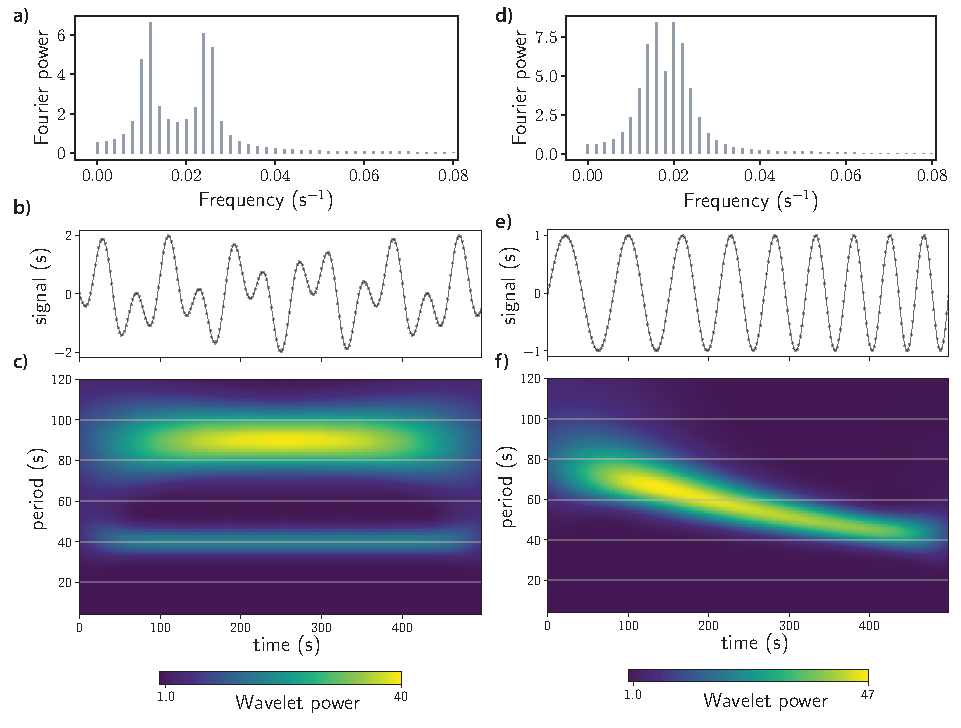
\includegraphics[width=\linewidth]{figures/Figure1}
\caption{a) Fourier power spectrum showing two peaks corresponding to the two harmonic components present in the signal.  b) Synthetic  signal is harmonic composition with two periods $T_1$ = 40s ($f_1$ = 0.025Hz) and $T_2$ = 90s ($f_2$ = 0.011Hz). c) Wavelet power spectrum, both harmonic components are prominently featured. d) Fourier power spectrum shows a range of frequencies but no information about their time dependence. e) Synthetic signal sweeps linearly from $T_2$ to $T_1$. f) Wavelet power spectrum shows time-resolved (instantaneous) periods. }
\label{fig1}
\end{figure}

Mathematically, decompositions of the form of equation \ref{Ftrafo} work by choosing a specific set of \textit{basis functions}. For the Fourier transform, these basis functions are the Sines and Cosines which have no \textit{localization in time} but are sharply \textit{localized in frequency}. Each harmonic component carries exactly one frequency effective everywhere in time. The idea to reach an optimal compromise between time and frequency localization goes back to Gabor (\cite{Gabor1946}). He introduced Gaussian modulated harmonic components:
\begin{align}
  \Psi(t) &= \pi^{-1/4} \; e^{-t^2/2} \; e^{i\omega_0 t}\\
  &= \pi^{-1/4} \; e^{-t^2/2} \; \left[cos(\omega_0 t) + i\; sin(\omega_0 t) \right]
\end{align}
This function is also known as \textit{Morlet wavelet}. The basis function for time-frequency analysis are then generated from the \textit{mother wavelet} by \textit{scaling} and \textit{translation}:
\begin{equation}
  \Psi_{s,\tau}(t) = s^{-1/2}\;\Psi \lt(\frac{t - \tau}{s}\rt)
\end{equation}
Varying the time localization $\tau$ slides the wavelet left and right on the time axis. The scale $s$ changes the \textit{center frequency} of the Morlet wavelet according to $\omega_c(s) = \omega_0/s$ (see also Appendix \ref{cfreq}). Higher scales therefore generate wavelets with lower center frequency. The Gaussian envelope suppresses the harmonic component with frequency $\omega_c$ farer away from $\tau$, therewith localizes the wavelet in time. This frequency $\omega_c(s)$ is conventionally taken as the Fourier equivalent (or pseudo-) frequency of a Morlet wavelet with scale $s$. It's noteworthy to state that wavelets in general are not as sharply localized in frequency as their harmonic counterparts, it's a tradeoff necessary for the gain in time localization.

The wavelet transform of a signal $f(t)$ is given by the following integral expression:
\begin{equation}
\label{Wtrafo}
\mathcal{W}[f](\tau, s) = \int_{-\infty}^{\infty} f(t) \; s^{-1/2} \;
                    \Psi^* \lt(\frac{t - \tau}{s} \rt) dt
\end{equation}    
For a fixed scale, this equation has the form of a complex convolution. Computing this convolution for many scales constitutes the continuous wavelet transform. One useful interpretation of the formula above is to treat it as a cross-correlation between the signal and the wavelet of scale $s$ (or center frequency $\omega_c(s)$): the translation variable $\tau$ slides the wavelet along the signal, and as the wavelet decays fastly away from $\tau$ only the instantaneous correlation of the wavelet with center frequency $\omega_c$ and the signal around $\tau$ contributes to the integral. By using an array of wavelets with different frequencies, this allows to scan for multiple frequencies in the signal in a time-resolved manner (see Figure \ref{fig1}f).

The result of the transform: $\mathcal{W}: f(t) \rightarrow \widetilde{f}(\tau,\omega)$ is a complex valued function of two variables, frequency $\omega$ and time localization $\tau$. Here and in the following we implicitly convert scales to frequency via the corresponding central frequencies of the Morlet wavelets. (in our tool the user never has to deal with scales directly). To obtain a physically meaningful quantity, one now defines the \textit{wavelet power spectrum}:
\begin{equation}
P_\mathcal{W}(\tau, \omega) = \frac{|\widetilde{f}(\tau, \omega)|^2}{\sigma^2}
\end{equation}
By stacking the transformations frequency-ordered one constructs a two-dimensional ($\tau-\omega$) representation of the wavelet power spectrum, where the power itself is usually color coded (Figure \ref{fig1}c and f).


We adopted the normalization with the standard deviation of the signal $\sigma$ from ref. \cite{Torrence1998} as it allows for a natural and statistical interpretation of the wavelet power.

